\documentclass{article}
\usepackage{assignment_preamble}

\title{Homework 1}
\author{Ravi Kini}
\date{October 5, 2023}

\begin{document}

\maketitle

\problem[\textit{An Introduction to Thermal Physics} (Schroeder,  1e) Exercise 1.16, 1.40]
\subproblem{(a)}
We consider a horizontal slab of air with thickness $\diff{z}$.

\begin{center}
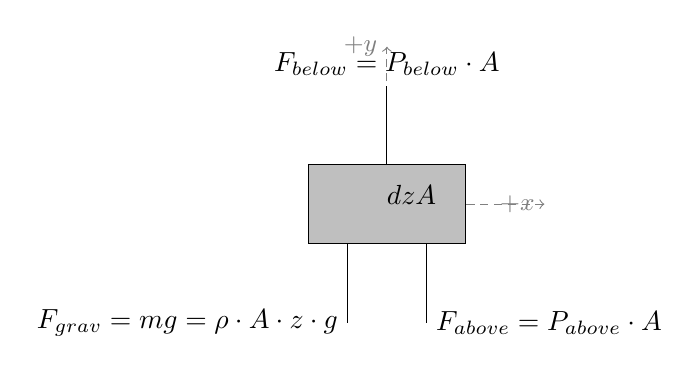
\begin{tikzpicture}[
    force/.style={>=latex,draw=blue,fill=blue},
    axis/.style={densely dashed,gray,font=\small},
    m_2/.style={rectangle,draw=black,fill=lightgray,minimum height=1.0cm,minimum width=2.0cm,thin},
]

\node[m_2] (m_2) {};
    \draw[axis,->] (m_2) -- ++(0,2) node[left] {$+y$};
    \draw[axis,->] (m_2) -- ++(2,0) node[left] {$+x$};
    {[force,->]
        \draw (m_2.north) -- ++(0,1) node[above] {$F_{below} = P_{below} \cdot A$};
        \draw (m_2.south) ++(0.5,0) -- ++(0,-1) node[right] {$F_{above} = P_{above} \cdot A$};
        \draw (m_2.south) ++(-0.5,0) -- ++(0,-1) node[left] {$F_{grav} = mg = \rho \cdot A \cdot \diff{z} \cdot g$};
    }
    \dimline [extension start length=0.5, extension end length=0.5] {(-1.5,-0.5)}{(-1.5,0.5)}{$dz$};
    \dimline [extension start length=-0.25, extension end length=-0.25] {(-1,-1)}{(1,-1)}{$A$};

\end{tikzpicture}
\end{center}

Balancing forces on the slab:
\begin{equation}
    \begin{split}
        F_{\text{below}} & = F_{\text{above}} + F_{\text{grav}} \\
        P_{\text{below}} \cdot A & = P_{\text{above}} \cdot A + \rho \cdot A \cdot \diff{z} \cdot g \\
        P_{\text{below}} & = P_{\text{above}} + \rho \cdot \diff{z} \cdot g \\
        \diff{p} = P_{\text{above}} - P_{\text{below}} & = -\rho g \cdot dz \\
        \deriv{p}{z} & = -\rho g
    \end{split}
\end{equation}
\subproblem{(b)}
Assuming the dry air can be treated as an ideal gas, equating the mole fraction and volume fraction:
\begin{equation}
    \begin{split}
        m_{\ce{N2}} & = 0.78~\unit{\mole} \cdot 28.0134~\unit{\gram\per\mole} = 21.850452~\unit{\gram} \\
        m_{\ce{O2}} & = 0.21~\unit{\mole} \cdot 31.999~\unit{\gram\per\mole} = 6.71979~\unit{\gram} \\
        m_{\ce{Ar}} & = 0.01~\unit{\mole}\cdot 39.948~\unit{\gram\per\mole} = 0.39948~\unit{\gram} \\
        m_{\text{air}} & = m_{\ce{N2}} + m_{\ce{O2}} + m_{\ce{Ar}} = 28.969722~\unit{\gram}
    \end{split}
\end{equation}
One mole of dry air has a mass of $28.969722 \unit{\gram}$. One molecule of dry air then has a mass of $\frac{m_{\text{air}}}{N_A} = 4.810536 \cdot 10^{-26}~\unit{\kilo\gram}$.
\subproblem{(c)}
Using the ideal gas law:
\begin{equation}
    \begin{split}
        pV & = Nk_B T \\
        \rho = \frac{M}{V} & = \frac{mN}{\frac{Nk_B T}{p}} = \frac{mp}{k_B T} \\
        \deriv{p}{z} = -\rho g & = -\frac{mpg}{k_B T}
    \end{split}
\end{equation}
\subproblem{(d)}
Solving to find the differential equation of pressure as a function of height:
\begin{equation}
    \begin{split}
        \frac{1}{p} \, \diff{p} & = -\frac{mg}{k_BT} \, \diff{z} \\
        \int \frac{1}{p} \, \diff{p} & = \int -\frac{mg}{k_B T} \, \diff{z} \\
        \ln{p} & = -\frac{mgz}{k_B T} + C \\
        p\left(z\right) & = e^{-\frac{mgz}{k_B T} + C} = e^C e^{-\frac{mgz}{k_B T}} \\
        p\left(0\right) & = e^C e^{-\frac{mg\left(0\right)}{k_B T}} = e^C \\
        p\left(z\right) & = p\left(0\right)e^{-\frac{mgz}{k_B T}} \\
        \rho = \frac{mp}{k_B T} & = p\left(0\right)\frac{m}{k_B T}e^{-\frac{mgz}{k_B T}}
    \end{split}
\end{equation}
\subproblem{(e)}
\begin{equation}
    \begin{split}
        p(1430) & = p(0)e^{-\frac{mgz}{k_BT}} \\
        & = 1 \cdot e^{-\frac{4.810536 \cdot 10^{-26}~\unit{\kilo\gram} \cdot 9.8~\unit{\meter\per\second\squared} \cdot 1430~\unit{\meter}}{1.380649 \cdot 10^{-23}~\unit{\joule\per\kelvin} \cdot 300~\unit{\kelvin}}} \\
        & = 0.849794043523 \unit{atm} \\
    \end{split}
\end{equation}
Ogden (elevation $z \approx 1430~\unit{\meter}$) has an air pressure of $0.849794043523 \unit{atm}$.
\begin{equation}
    \begin{split}
        p(4420) & = p(0)e^{-\frac{mgz}{k_BT}} \\
        & = 1 \cdot e^{-\frac{4.810536 \cdot 10^{-26}~\unit{\kilo\gram} \cdot 9.8~\unit{\meter\per\second\squared} \cdot 4420~\unit{\meter}}{1.380649 \cdot 10^{-23}~\unit{\joule\per\kelvin} \cdot 300~\unit{\kelvin}}} \\
        & = 0.604665261999~\unit{atm} \\
    \end{split}
\end{equation}
Mt. Whitney (elevation $z \approx 4420~\unit{\meter}$) has an air pressure of $0.604665261999 \unit{atm}$.
\begin{equation}
    \begin{split}
        p(8840) & = p(0)e^{-\frac{mgz}{k_BT}} \\
        & = 1 \cdot e^{-\frac{4.810536 \cdot 10^{-26}~\unit{\kilo\gram} \cdot 9.8~\unit{\meter\per\second\squared} \cdot 8840~\unit{\meter}}{1.380649 \cdot 10^{-23}~\unit{\joule\per\kelvin} \cdot 300~\unit{\kelvin}}} \\
        & = 0.365620079068~\unit{atm} \\
    \end{split}
\end{equation}
Mt. Everest (elevation $z \approx 8840~\unit{\meter}$) has an air pressure of $0.365620079068~\unit{atm}$.
\subproblem{(f)}
Using the ideal gas law:
\begin{equation}
    \begin{split}
        pV & = Nk_B T \\
        \diff{(pV)} = p \, \diff{V} + V \, \diff{p} & = Nk_B \, \diff{T} \\
        -p \, \diff{V} & = V \, \diff{p} - Nk_B \, \diff{T} \\
        & = \frac{Nk_B T}{p} \, \diff{p} - Nk_B \, \diff{T} \\
    \end{split}
\end{equation}
Since the gas expands adiabatically:
\begin{equation}
    \begin{split}
        \diff{U} = W & = -p \, \diff{V} \\
        \frac{f}{2}Nk_B \, \diff{T} & = \frac{Nk_B T}{p} \, \diff{p} - Nk_B \, \diff{T} \\
        \frac{f + 2}{2} \, \diff{T} & = \frac{T}{p} \, \diff{p} \\
        \deriv{T}{p} & = \frac{2}{f + 2}\frac{T}{p}
    \end{split}
\end{equation}
\subproblem{(g)}
\begin{equation}
    \begin{split}
        \diff{T} & = \frac{2}{f + 2}\frac{T}{p} \, \diff{p} = -\frac{2}{f + 2}\frac{T}{p}\frac{mpg}{k_B T} \, \diff{z} = -\frac{2}{f + 2}\frac{mg}{k_B} \, \diff{z} \\
        \deriv{T}{z} & = -\frac{2}{f + 2}\frac{mg}{k_B} \\
        & = -\frac{2}{5 + 2}\frac{4.810536 \cdot 10^{-26}~\unit{\kilo\gram} \cdot 9.8~\unit{\meter\per\second\squared}}{1.380649 \cdot 10^{-23}~\unit{\joule\per\kelvin}} \\
        & = -0.00975591971602~\unit{\kelvin\per\meter} = -9.75591971602~\unit{\kelvin\per\kilo\meter}
    \end{split}
\end{equation}
The critical value of the temperature gradient is $\deriv{T}{z}= -9.75591971602~\unit{\kelvin\per\kilo\meter}$.

\clearpage

\problem[\textit{An Introduction to Thermal Physics} (Schroeder, 1e) Exercise 1.25]
Water molecules have three translational degrees of freedom corresponding to movement in the $x$-, $y$-, and $z$-directions. They are further nonlinear molecules, giving them three rotational degrees of freedom. The hydrogen atoms can each vibrate towards and away from the oxygen atom, or towards and away from each other, giving it six vibrational degrees of freedom for a total of twelve degrees of freedom.

\clearpage

\problem[\textit{An Introduction to Thermal Physics} (Schroeder, 1e) Exercise 1.16]
\subproblem{(a)}
The gas is ideal and monatomic, originally at a temperature $T_i$ and pressure $p_i$, and is compressed quasistatically to half its original volume and a final temperature $T_f$ such that at each instant, $p = AV^3$ for constant $A$. The $p$-$V$ diagram is then:
\begin{center}
    \begin{tikzpicture}
        \begin{axis}[samples=200,xlabel=$V$,ylabel=$p$,ytick={1,0.125},yticklabels={$p_i$, $p_f$},xtick={1,0.5},xticklabels={$V_i$, $V_f$},xmin=0,xmax=1.5,ymin=0,ymax=1.5]
        \addplot[color=black,domain=0.5:0.75]{x^3};
        \addplot[color=black,domain=0.75:1,<-]{x^3};
        \addplot[dashed,color=gray,domain=0:1.5]{1/x} node[above,pos=0.995] {$T_i$};
        \addplot[dashed,color=gray,domain=0:1.5]{1/(16*x)} node[above,pos=0.89] {$T_f$};
        \end{axis}
    \end{tikzpicture}
\end{center}
\subproblem{(b)}
Using the ideal gas law:
\begin{equation}
    \begin{split}
        \frac{p_iV_i}{T_i} & = Nk_B = \frac{p_fV_f}{T_f} \\
        \frac{p_i\sqrt[3]{\frac{p_i}{A}}}{T_i} & = \frac{(A \cdot \frac{1}{8}\frac{p_i}{A})\frac{1}{2}\sqrt[3]{\frac{p_i}{A}}}{T_f} \\
        T_f & = \frac{1}{16}T_i
    \end{split}
\end{equation}
\subproblem{(c)}
Using the fact that the compression is quasistatic, the work done $W$ is:
\begin{equation}
    \begin{split}
        W & = -\int_{V_i}^{V_f} P \, \diff{V} \\
        & = -\int_{V_i}^{\frac{1}{2}V_i} AV^3 \, \diff{V} \\
        & = \left.-\frac{AV^4}{4}\right\vert_{V_i}^{\frac{1}{2}V_i} = \frac{15A}{64}V_i^4 = \frac{15}{64}Nk_B T_i
    \end{split}
\end{equation}
\subproblem{(d)}
The change in energy of the gas $\diff{U}$ is:
\begin{equation}
    \begin{split}
        \diff{U} & = \frac{f}{2}Nk_B \, \diff{T} = -\frac{45}{32}Nk_B T_i
    \end{split}
\end{equation}
\subproblem{(e)}
The heat transferred from the gas to the environment $Q$ is:
\begin{equation}
    \begin{split}
        Q = \diff{U} - W & = -\frac{45}{32}Nk_B T_i - \frac{15}{64}Nk_B T_i = -\frac{105}{64}Nk_B T_i
    \end{split}
\end{equation}
\subproblem{(f)}
Heat was lost, and the temperature was not kept constant, so the process described is neither adiabatic nor isothermal.

\end{document}